\documentclass{article}\usepackage[]{graphicx}\usepackage[]{color}
%% maxwidth is the original width if it is less than linewidth
%% otherwise use linewidth (to make sure the graphics do not exceed the margin)
\makeatletter
\def\maxwidth{ %
  \ifdim\Gin@nat@width>\linewidth
    \linewidth
  \else
    \Gin@nat@width
  \fi
}
\makeatother

\definecolor{fgcolor}{rgb}{0.345, 0.345, 0.345}
\newcommand{\hlnum}[1]{\textcolor[rgb]{0.686,0.059,0.569}{#1}}%
\newcommand{\hlstr}[1]{\textcolor[rgb]{0.192,0.494,0.8}{#1}}%
\newcommand{\hlcom}[1]{\textcolor[rgb]{0.678,0.584,0.686}{\textit{#1}}}%
\newcommand{\hlopt}[1]{\textcolor[rgb]{0,0,0}{#1}}%
\newcommand{\hlstd}[1]{\textcolor[rgb]{0.345,0.345,0.345}{#1}}%
\newcommand{\hlkwa}[1]{\textcolor[rgb]{0.161,0.373,0.58}{\textbf{#1}}}%
\newcommand{\hlkwb}[1]{\textcolor[rgb]{0.69,0.353,0.396}{#1}}%
\newcommand{\hlkwc}[1]{\textcolor[rgb]{0.333,0.667,0.333}{#1}}%
\newcommand{\hlkwd}[1]{\textcolor[rgb]{0.737,0.353,0.396}{\textbf{#1}}}%
\let\hlipl\hlkwb

\usepackage{framed}
\makeatletter
\newenvironment{kframe}{%
 \def\at@end@of@kframe{}%
 \ifinner\ifhmode%
  \def\at@end@of@kframe{\end{minipage}}%
  \begin{minipage}{\columnwidth}%
 \fi\fi%
 \def\FrameCommand##1{\hskip\@totalleftmargin \hskip-\fboxsep
 \colorbox{shadecolor}{##1}\hskip-\fboxsep
     % There is no \\@totalrightmargin, so:
     \hskip-\linewidth \hskip-\@totalleftmargin \hskip\columnwidth}%
 \MakeFramed {\advance\hsize-\width
   \@totalleftmargin\z@ \linewidth\hsize
   \@setminipage}}%
 {\par\unskip\endMakeFramed%
 \at@end@of@kframe}
\makeatother

\definecolor{shadecolor}{rgb}{.97, .97, .97}
\definecolor{messagecolor}{rgb}{0, 0, 0}
\definecolor{warningcolor}{rgb}{1, 0, 1}
\definecolor{errorcolor}{rgb}{1, 0, 0}
\newenvironment{knitrout}{}{} % an empty environment to be redefined in TeX

\usepackage{alltt}
\usepackage{mathtools}

\renewcommand{\abstractname}{Overview}
\IfFileExists{upquote.sty}{\usepackage{upquote}}{}
\begin{document}
%\SweaveOpts{concordance=TRUE}







\title{Statistical Inference Project 2 Part 2}
\author{Nicolas Moreno Andrade}
% \date{}
\maketitle
\begin{abstract}
In this project we will study the ToothGrowth data set. This set contains data about the effect of vitamin C in tooth growth (measured by length) of guinea pigs. We'll perform some exploratory data analysis by performing quick summaries and drawing boxplots by dose level and delivery method. Additionaly t-tests will be run in order to confirm the relationships seen in the plots. At the end we will conclude that there is a positive and significant relationship between tooth growth and ingestion of vitamin C and no relationship with delivery method.   
\end{abstract}

\section{Basic Summary of Data}

The ToothGrowth data contains 60 observations of length of odontoblasts (cells responsible for tooth growth) in guinea pigs. Each animal received one of three dose levels of vitamin C (0.5, 1, and 2 mg/day) by one of two delivery methods, (orange juice or ascorbic acid (a form of vitamin C and coded as VC). 

The following are basic summaries of the data: 
\begin{knitrout}
\definecolor{shadecolor}{rgb}{0.969, 0.969, 0.969}\color{fgcolor}\begin{kframe}
\begin{alltt}
\hlkwd{summary}\hlstd{(ToothGrowth)}
\end{alltt}
\begin{verbatim}
##       len        supp         dose      
##  Min.   : 4.20   OJ:30   Min.   :0.500  
##  1st Qu.:13.07   VC:30   1st Qu.:0.500  
##  Median :19.25           Median :1.000  
##  Mean   :18.81           Mean   :1.167  
##  3rd Qu.:25.27           3rd Qu.:2.000  
##  Max.   :33.90           Max.   :2.000
\end{verbatim}
\begin{alltt}
\hlkwd{dim}\hlstd{(ToothGrowth)}
\end{alltt}
\begin{verbatim}
## [1] 60  3
\end{verbatim}
\begin{alltt}
\hlkwd{table}\hlstd{(ToothGrowth}\hlopt{$}\hlstd{dose, ToothGrowth}\hlopt{$}\hlstd{supp)}
\end{alltt}
\begin{verbatim}
##      
##       OJ VC
##   0.5 10 10
##   1   10 10
##   2   10 10
\end{verbatim}
\begin{alltt}
\hlkwd{str}\hlstd{(ToothGrowth)}
\end{alltt}
\begin{verbatim}
## 'data.frame':	60 obs. of  3 variables:
##  $ len : num  4.2 11.5 7.3 5.8 6.4 10 11.2 11.2 5.2 7 ...
##  $ supp: Factor w/ 2 levels "OJ","VC": 2 2 2 2 2 2 2 2 2 2 ...
##  $ dose: num  0.5 0.5 0.5 0.5 0.5 0.5 0.5 0.5 0.5 0.5 ...
\end{verbatim}
\end{kframe}
\end{knitrout}

\section{Analysis}
\begin{knitrout}
\definecolor{shadecolor}{rgb}{0.969, 0.969, 0.969}\color{fgcolor}\begin{kframe}
\begin{alltt}
\hlcom{# boxplot delivery methods}
\hlkwd{ggplot}\hlstd{(}\hlkwd{aes}\hlstd{(}\hlkwc{x}\hlstd{=supp,} \hlkwc{y}\hlstd{=len),} \hlkwc{data}\hlstd{=ToothGrowth)} \hlopt{+}
  \hlkwd{geom_boxplot}\hlstd{(}\hlkwd{aes}\hlstd{(}\hlkwc{fill}\hlstd{=supp))}\hlopt{+}
        \hlkwd{xlab}\hlstd{(}\hlstr{"Supplement type"}\hlstd{)} \hlopt{+}\hlkwd{ylab}\hlstd{(}\hlstr{"Tooth length"}\hlstd{)} \hlopt{+}
  \hlkwd{scale_fill_discrete}\hlstd{(}\hlkwc{name}\hlstd{=}\hlstr{"Delivery Method"}\hlstd{)}
\end{alltt}
\end{kframe}\begin{figure}[h]
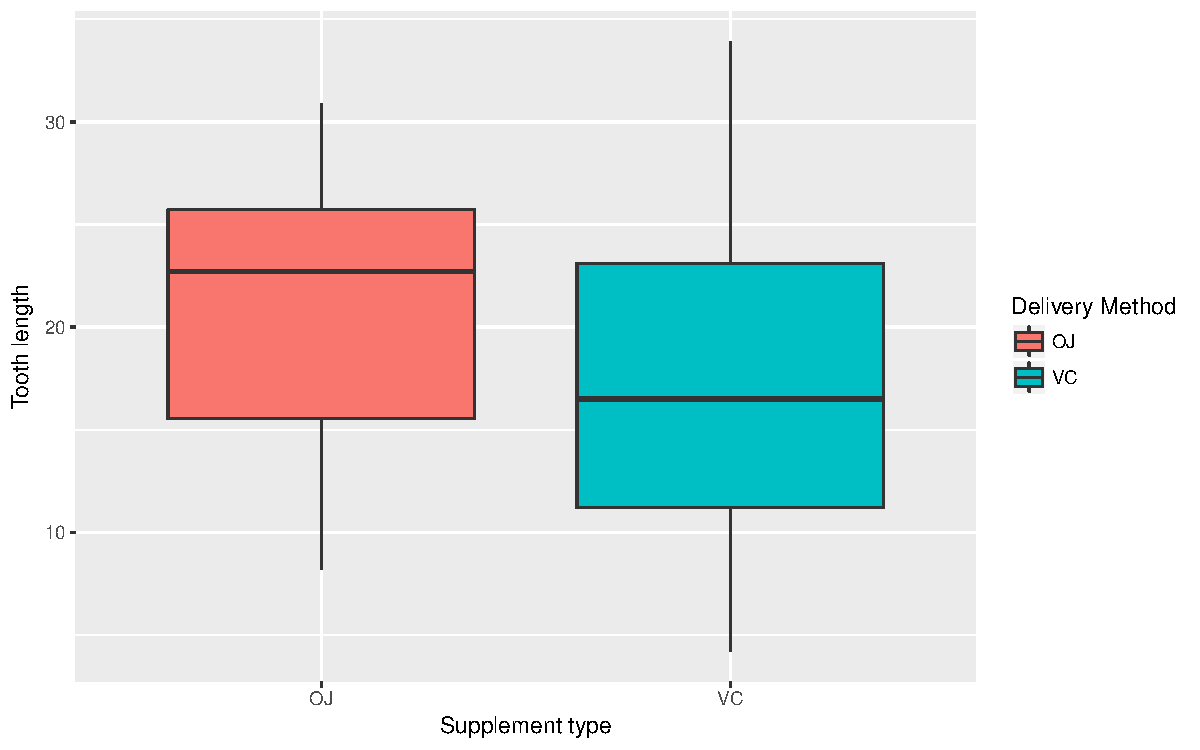
\includegraphics[width=\maxwidth]{figure/boxplot2-1} \caption[Boxplot comparing delivery methods by tooth length]{Boxplot comparing delivery methods by tooth length}\label{fig:boxplot2}
\end{figure}


\end{knitrout}

Based on this boxplot we see that dividing the observations just by delivery method doesn't seem to show relevant differences in tooth growth length. To confirm this we perform a t-test:

\begin{knitrout}
\definecolor{shadecolor}{rgb}{0.969, 0.969, 0.969}\color{fgcolor}\begin{kframe}
\begin{alltt}
\hlkwd{t.test}\hlstd{(len} \hlopt{~} \hlstd{supp,} \hlkwc{paired} \hlstd{=} \hlnum{FALSE}\hlstd{,} \hlkwc{var.equal} \hlstd{=} \hlnum{FALSE}\hlstd{,} \hlkwc{data} \hlstd{= ToothGrowth)}
\end{alltt}
\begin{verbatim}
## 
## 	Welch Two Sample t-test
## 
## data:  len by supp
## t = 1.9153, df = 55.309, p-value = 0.06063
## alternative hypothesis: true difference in means is not equal to 0
## 95 percent confidence interval:
##  -0.1710156  7.5710156
## sample estimates:
## mean in group OJ mean in group VC 
##         20.66333         16.96333
\end{verbatim}
\end{kframe}
\end{knitrout}

The confidence interval contains 0 and the p-value is greater than 0.05 so we fail to reject the null hypothesis. There is no significant difference in tooth length between the group that received the vitamin C in orange juice and the group that received it in the form of ascorbic acid.

\begin{knitrout}
\definecolor{shadecolor}{rgb}{0.969, 0.969, 0.969}\color{fgcolor}\begin{kframe}
\begin{alltt}
\hlcom{# boxplot dose}
\hlkwd{ggplot}\hlstd{(}\hlkwd{aes}\hlstd{(}\hlkwc{x}\hlstd{=}\hlkwd{factor}\hlstd{(dose),} \hlkwc{y}\hlstd{=len),} \hlkwc{data}\hlstd{=ToothGrowth)} \hlopt{+}
  \hlkwd{geom_boxplot}\hlstd{(}\hlkwd{aes}\hlstd{(}\hlkwc{fill}\hlstd{=}\hlkwd{factor}\hlstd{(dose)))}\hlopt{+}
        \hlkwd{xlab}\hlstd{(}\hlstr{"Dose"}\hlstd{)} \hlopt{+}\hlkwd{ylab}\hlstd{(}\hlstr{"Tooth length"}\hlstd{)} \hlopt{+}
  \hlkwd{scale_fill_discrete}\hlstd{(}\hlkwc{name}\hlstd{=}\hlstr{"Dose Level"}\hlstd{)}
\end{alltt}
\end{kframe}\begin{figure}[h]
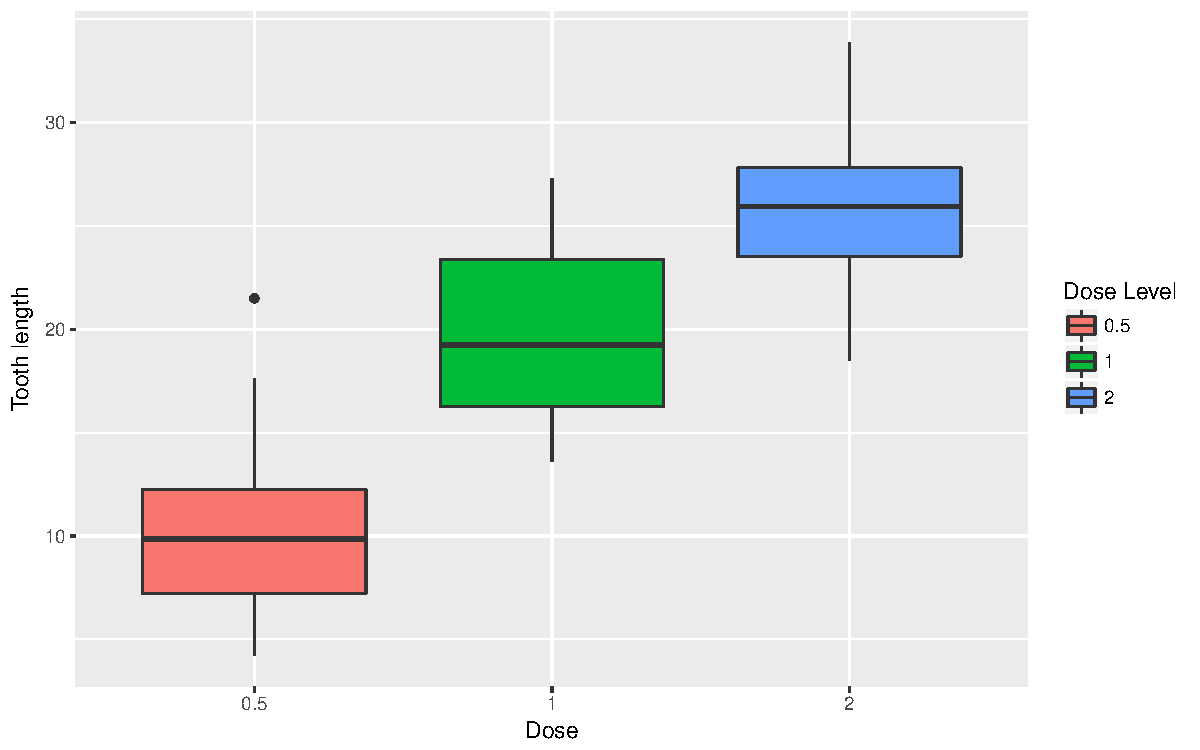
\includegraphics[width=\maxwidth,]{figure/boxplot1-1} \caption[Boxplot comparing dose by tooth length]{Boxplot comparing dose by tooth length}\label{fig:boxplot1}
\end{figure}


\end{knitrout}

The boxplot indicates that there could be a relationship between dosage and tooth length. The bigger the dose we see longer teeth in the animals.

We now perform a t-test for each dose level:

\begin{knitrout}
\definecolor{shadecolor}{rgb}{0.969, 0.969, 0.969}\color{fgcolor}\begin{kframe}
\begin{alltt}
\hlstd{dose05vsdose1} \hlkwb{<-} \hlstd{ToothGrowth[ToothGrowth}\hlopt{$}\hlstd{dose} \hlopt \hlkwd{c}\hlstd{(}\hlnum{0.5}\hlstd{,} \hlnum{1.0}\hlstd{), ]}
\hlstd{dose05vsdose2} \hlkwb{<-} \hlstd{ToothGrowth[ToothGrowth}\hlopt{$}\hlstd{dose} \hlopt \hlkwd{c}\hlstd{(}\hlnum{0.5}\hlstd{,} \hlnum{2.0}\hlstd{), ]}
\hlstd{dose1vsdose2} \hlkwb{<-} \hlstd{ToothGrowth[ToothGrowth}\hlopt{$}\hlstd{dose} \hlopt \hlkwd{c}\hlstd{(}\hlnum{1.0}\hlstd{,} \hlnum{2.0}\hlstd{), ]}
\hlkwd{t.test}\hlstd{(len} \hlopt{~} \hlstd{dose,} \hlkwc{paired} \hlstd{=} \hlnum{FALSE}\hlstd{,} \hlkwc{var.equal} \hlstd{=} \hlnum{FALSE}\hlstd{,} \hlkwc{data} \hlstd{= dose05vsdose1)}
\end{alltt}
\begin{verbatim}
## 
## 	Welch Two Sample t-test
## 
## data:  len by dose
## t = -6.4766, df = 37.986, p-value = 1.268e-07
## alternative hypothesis: true difference in means is not equal to 0
## 95 percent confidence interval:
##  -11.983781  -6.276219
## sample estimates:
## mean in group 0.5   mean in group 1 
##            10.605            19.735
\end{verbatim}
\end{kframe}
\end{knitrout}

\begin{knitrout}
\definecolor{shadecolor}{rgb}{0.969, 0.969, 0.969}\color{fgcolor}\begin{kframe}
\begin{alltt}
\hlkwd{t.test}\hlstd{(len} \hlopt{~} \hlstd{dose,} \hlkwc{paired} \hlstd{=} \hlnum{FALSE}\hlstd{,} \hlkwc{var.equal} \hlstd{=} \hlnum{FALSE}\hlstd{,} \hlkwc{data} \hlstd{= dose05vsdose2)}
\end{alltt}
\begin{verbatim}
## 
## 	Welch Two Sample t-test
## 
## data:  len by dose
## t = -11.799, df = 36.883, p-value = 4.398e-14
## alternative hypothesis: true difference in means is not equal to 0
## 95 percent confidence interval:
##  -18.15617 -12.83383
## sample estimates:
## mean in group 0.5   mean in group 2 
##            10.605            26.100
\end{verbatim}
\end{kframe}
\end{knitrout}

\begin{knitrout}
\definecolor{shadecolor}{rgb}{0.969, 0.969, 0.969}\color{fgcolor}\begin{kframe}
\begin{alltt}
\hlkwd{t.test}\hlstd{(len} \hlopt{~} \hlstd{dose,} \hlkwc{paired} \hlstd{=} \hlnum{FALSE}\hlstd{,} \hlkwc{var.equal} \hlstd{=} \hlnum{FALSE}\hlstd{,} \hlkwc{data} \hlstd{= dose1vsdose2)}
\end{alltt}
\begin{verbatim}
## 
## 	Welch Two Sample t-test
## 
## data:  len by dose
## t = -4.9005, df = 37.101, p-value = 1.906e-05
## alternative hypothesis: true difference in means is not equal to 0
## 95 percent confidence interval:
##  -8.996481 -3.733519
## sample estimates:
## mean in group 1 mean in group 2 
##          19.735          26.100
\end{verbatim}
\end{kframe}
\end{knitrout}


The three t-tests show similar results. The confidence intervals do not contain 0 and the p-value is very small (almost 0). We conclude that the mean tooth length increases with larger dose levels. 

\section{Conclusions}
\begin{enumerate}
\item The data indicates that, in guinea pigs,  mean tooth length increases with larger dose levels of vitamin C.
\item The delivery method does not seem to have a relationship with mean growth length.
\end{enumerate}

\section{Assumptions}
\begin{enumerate}
\item The 60 guinea pigs are a representative sample of the population of the guinea pigs.
\item We assumed unequal variance for the t-tests.
\end{enumerate}


  
\end{document}
